\chapter{Progettazione e scelte architetturali}

\section{Architettura}
\subsection{Visione statica del sistema: Component Diagram}
Progettazione della suddivisione per proprietà logice dei vari moduli del sistema.
\begin{itemize}
    \item Topologia del sistema:
    \begin{figure}[H]
        \centering
        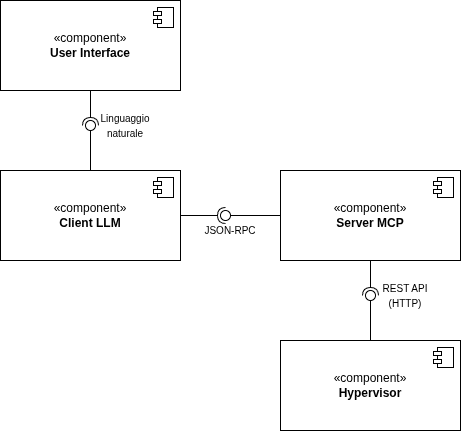
\includegraphics[width=0.7\textwidth]{assets/component_diagram.drawio.png}
        \caption{Component Diagram dell'intero sistema.}
        \label{fig:architettura_generale}
    \end{figure}

    \item Architettura interna del Middleware (MCP):
    \begin{figure}[H]
        \centering
        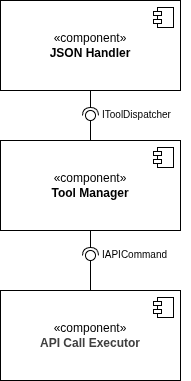
\includegraphics[width=0.3\textwidth]{assets/component_diagram_mcp.drawio.png}
        \caption{Component Diagram del Server MCP.}
        \label{fig:architettura_server_mcp}
    \end{figure}

    Come illustrato nel diagramma dei componenti interni (Figura \ref{fig:architettura_server_mcp}), il Server MCP è progettato seguendo un approccio modulare per la separazione delle responsabilità di parsing, logica applicativa e comunicazione di rete. Esso si articola in tre componenti logici sequenziali:
    \begin{itemize}
        \item \textbf{JSON Handler:} Costituisce il punto di ingresso del middleware. Ha il compito di intercettare il flusso di dati dal Client LLM, validare la conformità del messaggio allo standard JSON-RPC e verificare che i parametri forniti rispettino i \textit{JSON Schema} attesi. Una volta validato, il payload viene decodificato e inoltrato al livello logico successivo attraverso l'interfaccia \texttt{IToolDispatcher}.
        
        \item \textbf{Tool Manager:} Rappresenta il \textit{core} logico del sistema. Riceve la richiesta strutturata e si occupa di validarne il contesto operativo. In questo modulo risiede la logica di controllo degli accessi e l'implementazione del pattern \textit{Human-in-the-Loop}: se il tool richiesto prevede un'azione classificabile come distruttiva, il manager sospende l'esecuzione e genera una richiesta di conferma. Superati i controlli, formula il comando di backend e lo delega tramite l'interfaccia \texttt{IAPICommand}.
        
        \item \textbf{API Call Executor:} È il modulo incaricato dell'interazione con l'esterno. Riceve il comando astratto dal Tool Manager e lo traduce in chiamate HTTP/REST autenticate verso l'Hypervisor. Questo componente gestisce la latenza di rete, cattura le eccezioni o i codici di errore HTTP e si occupa di impacchettare le metriche ricevute in un' \textit{Observation} restituibile a ritroso fino all'LLM.
    \end{itemize}
\end{itemize}

\subsection{Visione dinamica del sistema: Sequence Diagram}
Di seguito una panoramica del flusso di funzionamento del sistema tramite la rappresentazione del Sequence Diagram del (\textit{UC3 - Esecuzione controllata di operazioni critiche}), in modo da poter prendere visione di una delle casistiche più complesse e cruciali del sistema:
\begin{figure}[H]
    \centering
    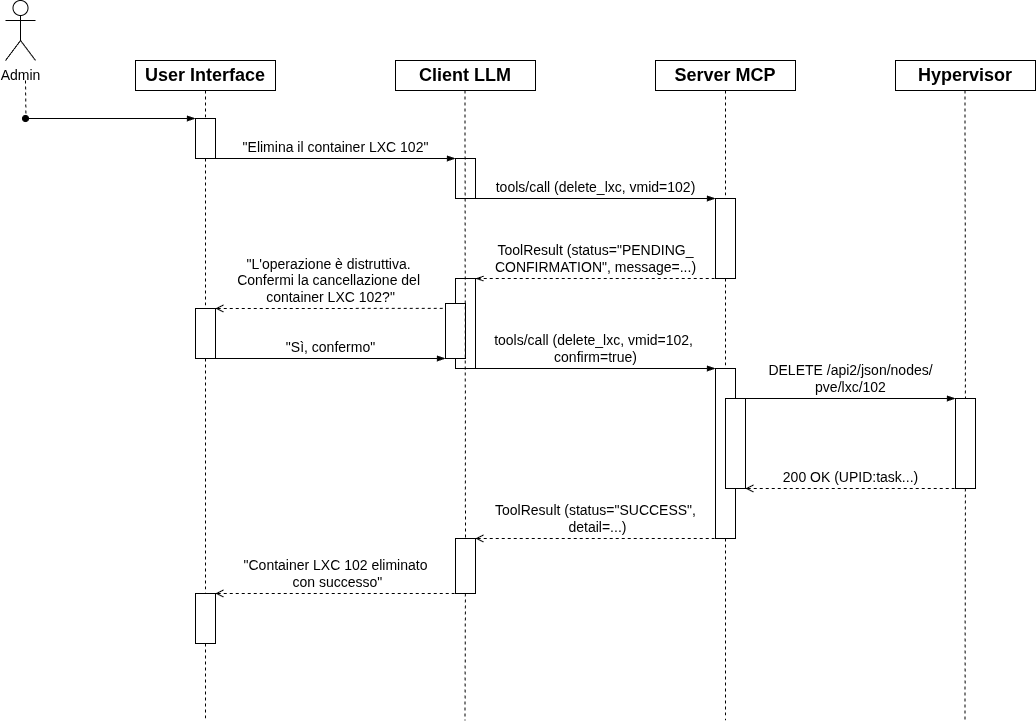
\includegraphics[width=1\textwidth]{assets/sequence_diagram_uc3.drawio.png}
    \caption{Sequence Diagram dell'UC3}
    \label{fig:sequence_diagram_uc3}
\end{figure}

\subsection{Modello di Comunicazione}
I dati attraversano la pipeline dei moduli tramite diversi cambi di protocollo affinchè ogni modulo possa interpretare le richieste in modo corretto.
\begin{itemize}
    \item \textbf{Utente $\longleftrightarrow$ Client LLM (Linguaggio Naturale):} L'interazione avviene tramite l'interfaccia conversazionale; l'operatore esprime gli intenti operativi o di diagnostica senza dover conoscere la sintassi delle API sottostanti.
    
    \item \textbf{Client LLM $\longleftrightarrow$ Server MCP (Protocollo JSON-RPC 2.0):} Il modello linguistico converte l'intento dell'utente in invocazioni strutturate di tool (\textit{Tool Calls}) serializzate in payload JSON-RPC conformi alla specifica MCP, scambiate tipicamente tramite canali di standard I/O (\texttt{stdio}) o Server-Sent Events (SSE).
    
    \item \textbf{Server MCP $\longleftrightarrow$ Hypervisor Proxmox VE (REST API su HTTPS):} Il middleware traduce le chiamate JSON-RPC ricevute in richieste HTTP formalizzate (verbi \texttt{GET}, \texttt{POST}, \texttt{PUT}, \texttt{DELETE}) indirizzate agli endpoint dell'API REST di Proxmox VE, includendo nei relativi header le credenziali di autenticazione (\textit{API Token}).
\end{itemize}

\section{Scelte progettuali}
A questo punto è necessario introdurre lo stack tecnologico di implementazione e di ambiene:
\begin{itemize}
    \item textbf{Python 3.11+: } La scelta sul linguaggio di sviluppo per il Server MCP è ricaduta su \textbf{Python} (versione 3.11+) per la sua ricca disponibilità di librerie 
\end{itemize}
